\subsection{Estudo de técnicas de reconhecimento} 

As informações de distância recebidas pelos sensores descritos na seção
anterior podem ser armazenados como uma estrutura de dados chamada nuvem de
pontos, isto é, uma representação tridimensional do espaço cartesiano, na qual cada distância medida pelos
sensores a partir de sua origem representa uma coordenada x y z.
Entretanto, essa representação não é capaz de diferenciar, ou classificar, os
limites de cada objeto presente na cena, ou seja, não é possível determinar
\textit{a priori} qual conjunto de pontos pertence a cada elemento que se deseja
identificar para a realização da calibração.

A identificação de cada conjunto, ou \textit{cluster}, de pontos é importante
para que a posição e orientação de cada objeto de interesse seja determinada e,
assim a transformação do sistema de coordenadas entre cada objeto seja
calculada. Esse processo necessita, então, do estudo e implementação de
algoritmos para a análise da nuvem de pontos, identificação dos elementos
necessários, extração de suas respectivas posições e, finalmente, cálculo da
transformação entre as posições. 

Dependendo das características de cada objeto a ser identificado e da
possibilidade de implementação de uma estrutura de apoio para facilitar a sua
identificação, podem ser utilizados diferentes métodos e estratégias de
identificação e localização, que serão exploradas a seguir.

\subsubsection{Reconhecimento do Robô}

O Robô é uma estrutura que a idenficação pode ser facilitada pelo uso de
padrões de fácil reconhecimento (como esferas e padrões de xadrez ), pois
alterações na base do robô não ocasionam problemas para o funcionamento do sistema.

Devido a baixa iluminação ambiente dentro do circuito da tubina, a opção
mais simples é o uso de nuvem de pontos sem identificação de cor. Ou seja, o
reconhecimento se dará apenas pelo formato 


\subsubsection{Reconhecimento da Pá} 

Para a identificação e localização das pás das turbinas não é possível a
utilização de algum artifício de apoio que facilite o processamento da nuvem de
pontos, pois a instalação de qualquer um desses aparatos não pode ter precisão
garantida nas operações de campo. Uma instalação de um elemento de apoio em
pontos precisos da pá necessitaria também de calibração para cada utilização, retirando assim
o propósito do método. 

Portanto, para a localização das pás da turbina é
necessário explorar as características espaciais intrínsecas à superfície do
próprio objeto e identificá-las na nuvem de pontos do ambiente. O objetivo
principal nessa etapa do processo é, então, identificar um conjunto mínimo de
características do objeto que represente unicamente o mesmo, com um baixo grau
de ambiguidade e sem exigir muito esforço computacional. 

A escolha do tipo de característica a se usar é uma decisão fundamental para a
eficiência do processo e tem sido alvo de estudos na literatura para a análise
e reconhecimentos de imagens 2D, como imagens RGB de câmeras e mais recentemente
também para imagens 3D. 

Uma boa representação de \textit{point feature} deve ser capaz de capturar as
mesmas características locais da superfície na presença de:

\begin{itemize}
  \item \textbf{Transformadas} -  rotações e translações 3D nos dados não devem
  influenciar a estimação dos descriptors;
  \item \textbf{Variações na densidade de amostragem} - em princípio, uma de
  superfície amostrada mais ou menos densamente deve ter a mesma assinatura característica do vetor
  \item \textbf{Ruído}
\end{itemize}

Na literatura, o reconhecimento de objetos em aplicações robóticas vem recebido
grande atenção, principamente com o crescimento da robótica móvel e em ambientes
não estruturados, onde é necessário identificar e localizar os objetos a serem
manipulados em cada tarefa. O problema é enfrentado basicamente utilizando-se
duas abordagens: analisar os dados 3D ou realizar algum tipo de processamento e
projeção para se trabalhar com imagens 2D e utilizar as técnicas mais maduras
desse tipo de imagem.

Nesta última categoria, a técnica de projeção
mais usada é converter as informações tridimensionais em \textit{Range Images},
na qual é realizada uma projeção a partir de um ponto de vista (geralmente o do sensor) e utiliza escala
de cores ou cinza para representar a distância, ou seja, quanto mais escuro o
objeto na imagem, mais longe ele se encontra. É importante reassaltar que esse
tipo de método introduz perdas de informação ao se realizar projeções e é
sensível à escolha do ponto de vista escolhido. Em \cite{Bayramoglu2010} são
utilizados descritores SIFT, ou \textit{Scale-Invariant Feature Transform},  
como características a serem identificadas na imagem. \textit{Local Feature
Histograms} são utilizados em \cite{Hetzel2001} e por sua vez \cite{Chen2007}
optou por utilizar \textit{Local surface patches}. A escolha do descritor a ser
utilizado depende da aplicação e deve ser estudada a melhor opção para a nossa
solução, assim que tivermos dados aquisitados pelo sensor. Uma comparação dos
descritores utilizados para reconhecimento de objetos 2D e 3D pode ser
encontrado em \cite{Zaharia2004, Weber2014}.

Após o reconhecimento do objeto, é necessário identificar a posição do mesmo. Em
\cite{Steder2009}, o alinhamento é realizado utilizando-se a própria
\textit{Range Image} e a informação de profundidade presente na mesma. Por outro
lado, em \cite{Nuchter2005} a região onde o objeto identificado está presente é
selecionada e, por meio de \textit{raycasting}, o conjunto de pontos da nuvem
pertecentes a essa região é identificado. Após essa segmentação, é utilizado um
algoritmo de alinhamento como o ICP.

O primeiro passo para ser possível localizar a pá é a aquisição de seus dados
espacias e a criação de uma nuvem de dados que represente a pá. A figura
\ref{fig::pa_pcd} ilustra uma nuvem de pontos representando uma pá de uma das
turbinas da usina de Jirau, esse modelo foi construído utilizando-se os dados
aquisitados durante a viagem de campo e teste de sensibilidade do sensor Faro
Focus X330 à umidade. É importante ressaltar que o modelo deve representar, se
possível, todas as características pertinentes do objeto de interesse. Nesse
sentido, se faz necessário a criação de um modelo para cada tipo de pá que
deverá ser processada. 


\begin{figure}[h!]
   \centering
   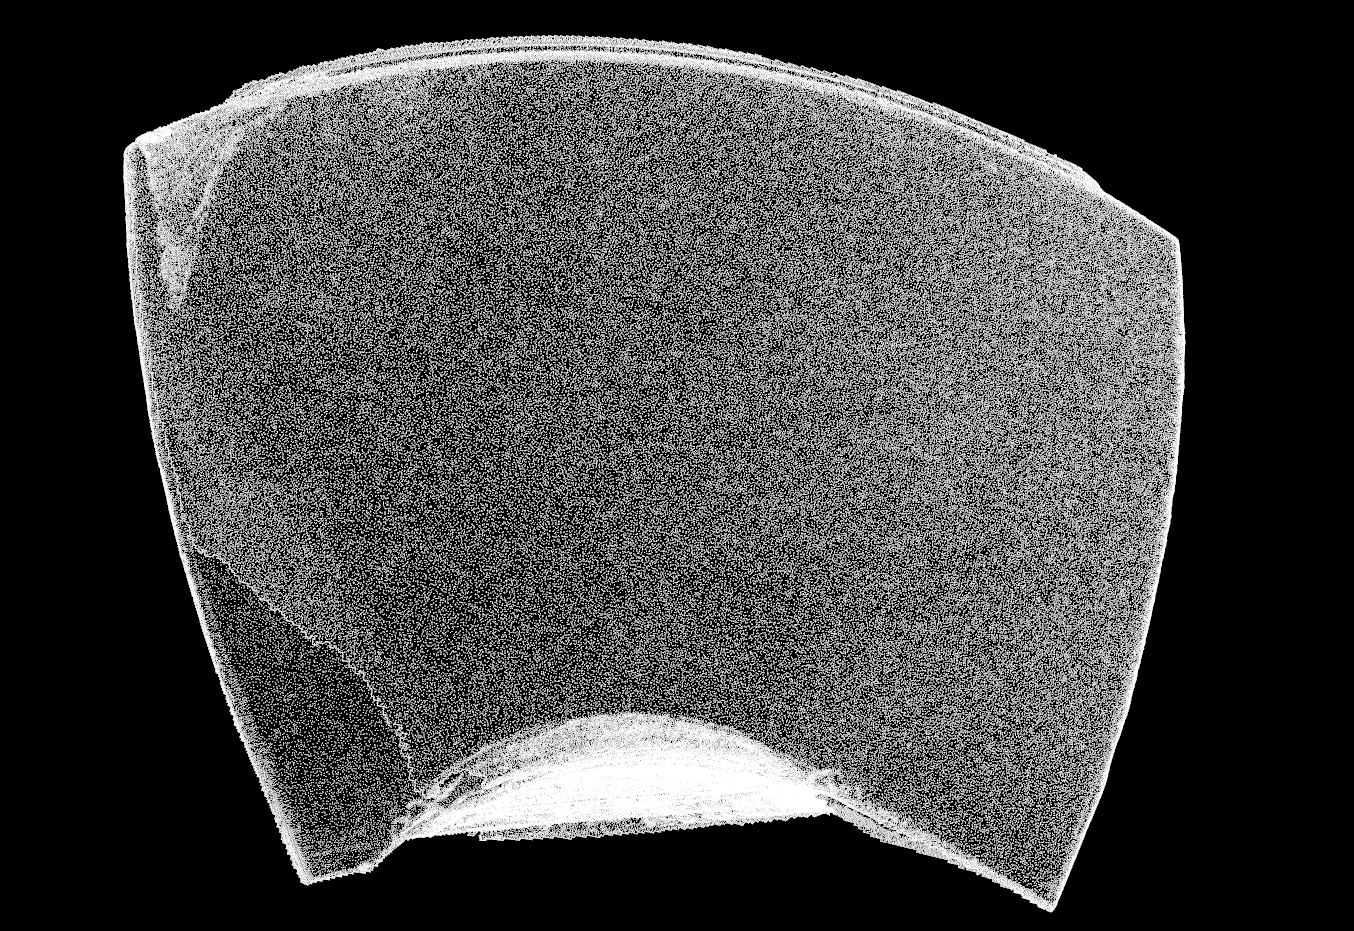
\includegraphics[width=0.95\columnwidth]{figs/localizacao/pa_pcd}
   \caption{Modelo da pá em nuvem de pontos}
   \label{fig::pa_pcd}
\end{figure}

A partir do modelo, é necessário a extração de seus pontos chaves e descritores.
A figura \ref{fig::pa_key} ilustra descritores do tipo SHOT, (explicação),
identificados no modelo de referência da pá. Para a nossa aplicação, não é
necessário, a princípio, o reconhecimento do objeto em questão, apenas a sua
localização e orientação no espaço tridimensional. A possibilidade de inserir no
sistema a informação de qual modelo de pá o sistema deve procurar, simplifica o
algoritmo e o torna menos suscetível a erros, uma vez o sistema não precisa
avaliar qual o modelo mais próximo das medições atuais e pode ainda nos
fornecer uma medida de avalição de quão bom está a similaridade do modelo com
os dados reais.

\begin{figure}[h!]
   \centering
   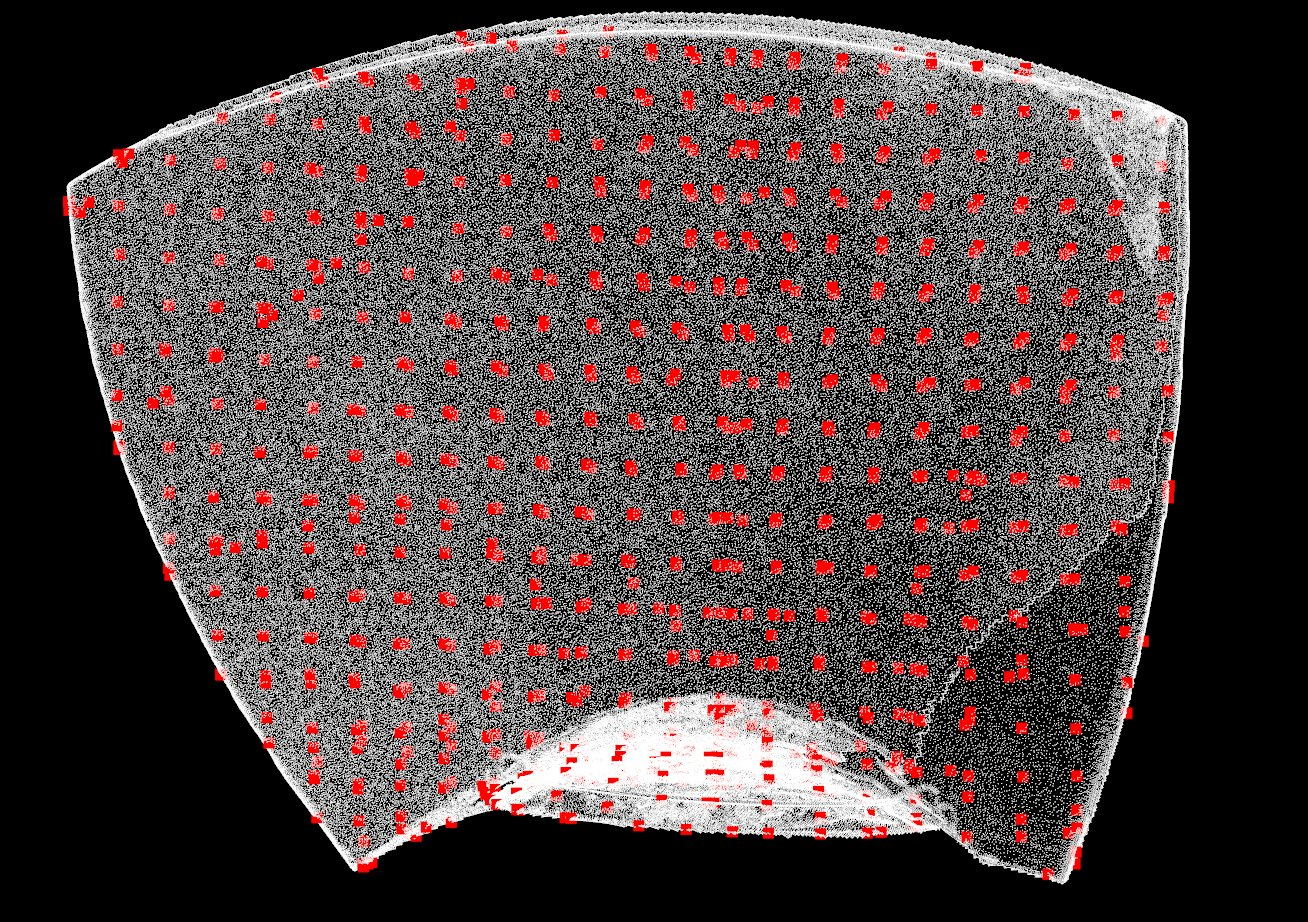
\includegraphics[width=0.95\columnwidth]{figs/localizacao/pa_key}
   \caption{Modelo da pá em nuvem de pontos}
   \label{fig::pa_key}
\end{figure}


Hough Voting - Tombari2010a
			  
			  
Correspondence Grouping




\subsubsection{Reconhecimento do Robô}